\section[Phylogenetic Clustering (Phyloclustering)]{Phylogenetic Clustering (Phyloclustering)}
\label{sec:phyloclustering}
\addcontentsline{toc}{section}{\thesection. Phylogenetic Clustering (Phyloclustering)}

Phylogenetic clustering (phyloclustering) is an evolutionary
Continuous Time Markov Chain (CTMC) model-based approach to identify population
structure from molecular data without assuming linkage equilibrium.
\begin{comment}
The \pkg{phyclust} package provides a convenient implementation of
phyloclustering for DNA and SNP data, capable of clustering individuals into
subpopulations and identifying molecular sequences representative
of those subpopulations.
It is designed in \proglang{C} for performance,
interfaced with \proglang{R} for visualization,
and incorporates other popular open source software for
simulating data and additional analyses.
All aspects are intended to make the software useful to a broad
spectrum of biological users.
\end{comment}
Let $\vect{X} = (x_{nl})_{N\times L}$ be the data matrix containing
$N$ sequences observed at $L$ sites. Denote the molecular sequence
of individual $n$ as
$\vect{x}_n = (x_{n1}, \ldots, x_{nL}) \in \mathfrak{X}$ and
$x_{nl} \in \mathcal{S}$ where
$\mathfrak{X}$ contains all possible sequences of length $L$ from alphabet
$\mathcal{S}$, e.g.\ $\mathcal{S} = \{\mbox{A}, \mbox{G}, \mbox{C}, \mbox{T}\}$
for nucleotide sequences.
A finite mixture model provides a statistical framework for clustering.
In this setting, each individual sequence $\vect{x}_n$ is independent
and identically drawn from
$
f(\vect{x}_n | \vect{\eta}, \vect{\Theta}) =
\sum_{k = 1}^K \eta_k f_k(\vect{x}_n | \Theta_k)
$
where $f_k()$ is the density for the $k$th component,
$\vect{\eta} = \{\eta_1, \ldots, \eta_K\}$ are the mixing proportions
summing to one, and
$\vect{\Theta} = \{\Theta_1,\ldots,\Theta_K\}$ contains parameters for the
components \citep{Fraley2002}.
Component $f_k()$ is modeled as a transition probability
$p_{\vect{\mu}_k,\vect{x}_n}(t_k)$ from a CTMC mutation
process \citep{Felsenstein2004}, where
a sequence $\vect{x}_n$ evolves from
an ancestor
$\vect{\mu}_k = (\mu_{k1}, \ldots, \mu_{kL}) \in \mathfrak{X}$
representing the $k$th cluster.
The evolutionary process is modeled with instantaneous rate matrix
$\vect{Q}_k$ and time $t_k$
which are allowed to differ by cluster, so that
$\Theta_k = \{\vect{\mu}_k, \vect{Q}_k, t_k\}$.
The likelihood is maximized by an EM algorithm \citep{Dempster1977},
sequences are classified
by the maximum posterior probabilities, and the number of clusters is
assessed by bootstrap \citep{Maitra2010}.

Available choices for the $Q_k$ parameterization in \pkg{phyclust} include
\code{JC69} \citep{Jukes1969}, \code{K80} \citep{Kimura1980},
and \code{HKY85} \citep{Hasegawa1985}.
These choices are listed in \code{.substitution.model}.
In addition, $Q_k$ and $t_k$ can be constrained across clusters as shown
in Table~\ref{tab:identifier} (also see \code{.identifier}).
\begin{table}[h]
\begin{center}
\caption{Combinations of Models}
\begin{tabular}{ccc} \hline\hline
Identifier & $\vect{Q}$ & $t$ \\ \hline
\code{EE}  & $\vect{Q}_1 = \vect{Q}_2 = \cdots = \vect{Q}_K$
           & $t_1 = t_2 = \cdots = t_K$ \\
\code{EV}  & $\vect{Q}_1 = \vect{Q}_2 = \cdots = \vect{Q}_K$
           & $t_1 \neq t_2 \neq \cdots \neq t_K$ \\
\code{VE}  & $\vect{Q}_1 \neq \vect{Q}_2 \cdots \neq \vect{Q}_K$
           & $t_1 = t_2 = \cdots = t_K$ \\
\code{VV}  & $\vect{Q}_1 \neq \vect{Q}_2 \neq \cdots \neq \vect{Q}_K$
           & $t_1 \neq t_2 \neq \cdots \neq t_K$ \\
\hline\hline
\end{tabular}
\label{tab:identifier}
\end{center}
\end{table}

The available initialization methods (\code{.init.method})
for the EM algorithm use pairwise distances, and
the available models for computing the 
evolutionary distance are listed in \code{.edist.model}.
The model used for computing distances need not match the model
used to model evolution in phylogenetic clustering (in \code{.substitution.model}).
There are additional pairwise distance models available
in the \pkg{ape} package \citep{Paradis2004}.

The \code{.show.option()} function lists all options
available in the \pkg{phyclust} package.
These options can be used in the \code{.EMControl()} function
to generate an options object (such as \code{.EMC}), which defines
the selected phyloclust model, the initialization method, the EM algorithm and
the data type.  This argument is passed to function \code{phyclust()} using argument \code{EMC}.
All options are explained in the help pages.
The best choices for options may vary with application.
In particular, initialization can be tricky, and you should try
several initialization algorithms (see Section~\ref{sec:emcontrol}).
\begin{Code}
> .show.option()
boundary method: ADJUST, IGNORE
code type: NUCLEOTIDE, SNP
edist model: D_JC69, D_K80, D_HAMMING
em method: EM, ECM, AECM
identifier: EE, EV, VE, VV
init method: randomMu, NJ, randomNJ, PAM, K-Medoids, manualMu
init procedure: exhaustEM, emEM, RndEM, RndpEM
standard code: 
     nid code code.l
[1,]   0    A      a
[2,]   1    G      g
[3,]   2    C      c
[4,]   3    T      t
[5,]   4    -      -
     sid code
[1,]   0    1
[2,]   1    2
[3,]   2    -
substitution model: 
          model  code.type
 [1,]      JC69 NUCLEOTIDE
 [2,]       K80 NUCLEOTIDE
 [3,]       F81 NUCLEOTIDE
 [4,]     HKY85 NUCLEOTIDE
 [5,]  SNP_JC69        SNP
 [6,]   SNP_F81        SNP
 [7,]     E_F81 NUCLEOTIDE
 [8,]   E_HKY85 NUCLEOTIDE
 [9,] E_SNP_F81        SNP
\end{Code}




\subsection[Exploring data]{Exploring data}
\label{sec:illustrate}
\addcontentsline{toc}{subsection}{\thesubsection. Exploring data}

\pkg{Phyclust} has functions to help visualize large datasets.
We have prepared a simulated dataset (\code{seq.data.toy}) with 100 nucleotide sequences of length 200 sites from 4 clusters.
The ancestral sequences were simulated using the HKY85 model \citep{Hasegawa1985} along a tree of height $0.15$ (expected number of mutations per site).
The observed sequences were simulated along independent trees with height $0.09$ descending from the ancestors.

We use \code{X} to indicate the data
and \code{X.class} to indicate the classification which can be
a result (\code{class.id}) of the \code{phyclust()} function
or known, in the case of simulation (\code{ms+seqgen}).
The \pkg{ms}+\pkg{seq-gen} simulation procedure within \pkg{phyclust} produces 
sequences with names \\
``\code{sequence.id-class.id},'' so the \proglang{R}
function \code{gsub()} (for details, type \code{?gsub}) can be used
to extract the sequence classification (\code{class id}).
In this section, we demonstrate visualization of a simulated dataset, where
the clusters are know. 
Similar figures can be produced for real datasets with clusters estimated by \code{phyclust()}.

The following code produces the plot of Figure~\ref{fig:toydots}.
Each row represents a sequence and each column represents a site.
By default, it will show all changes with respect to the consensus sequence.
If the \code{X.class} is omitted, then it draws in the original order of data,
otherwise in the cluster order.
\begin{Code}
> seq.data.toy
code.type: NUCLEOTIDE, n.seq: 100, seq.len: 200.
> X <- seq.data.toy$org
> X.class <- as.numeric(gsub(".*-(.)", "\\1", seq.data.toy$seqname))
> plotdots(X, X.class)
\end{Code}

The chosen sequence is fully colored, with green, blue, purple and red representing 
nucleotides A, G, C, and T.
All other sequences show only mutant sites compared to the consensus sequence.
The dashed lines separate the clusters.
The bottom row indicates the segregating sites, i.e.\ those sites containing
at least one mutation.
By default {\it only} segregating sites are shown.
Type \code{?plotdots} for more information.
\begin{figure}[h]
\begin{center}
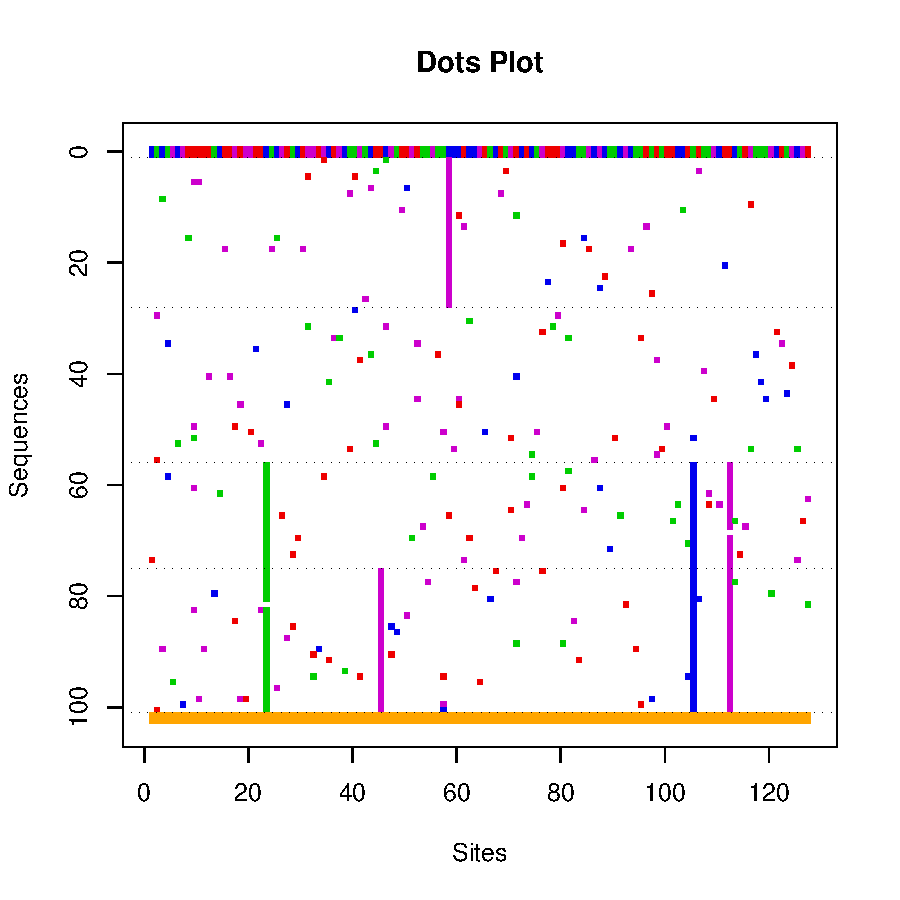
\includegraphics[width=5.0in]{./phyclust-include/f-toydots}
\caption{A dot plot for the toy dataset.}
\label{fig:toydots}
\end{center}
\end{figure}

Next, we may wish to see how many mutations each sequence has relative to a reference sequence.
The following code prepares the plot of Figure~\ref{fig:toyhist}, showing the number of mutations of all sequences within each cluster relative to the chosen reference sequence.
The top plot is for the whole dataset.
The other plots are for the four clusters.
\begin{Code}
> plothist(X, X.class)
\end{Code}
\begin{figure}[h]
\begin{center}
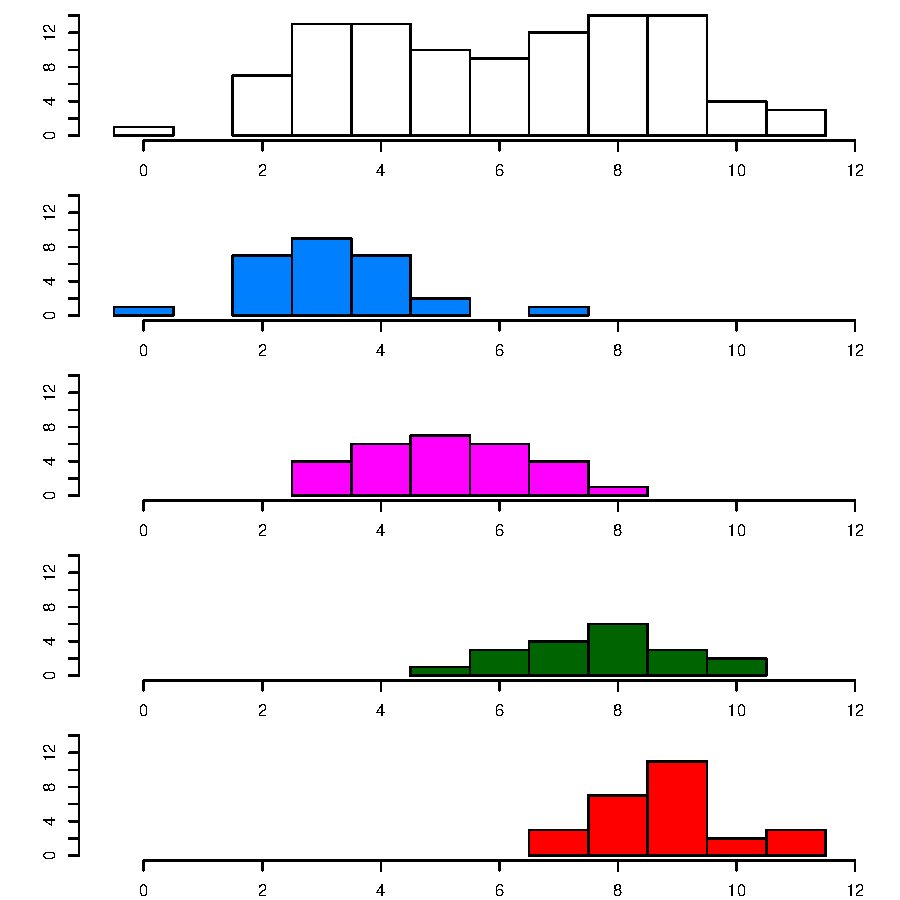
\includegraphics[width=5.0in]{./phyclust-include/f-toyhist}
\caption{A histogram plot for the toy dataset.}
\label{fig:toyhist}
\end{center}
\end{figure}

Last, we may like to visualize clusters on a more traditional diagram of evolutionary relationships, the phylogenetic tree.
The following code produces Figure~\ref{fig:toynj}.
The \code{phyclust.edist()} function takes in a data
matrix \code{X}, computes and returns pairwise distances for all sequences
using the Hamming distance
as a distance measure (\code{.edist.model[3]} is \code{D_HAMMING}).
The neighbor-joining method \citep{Saitou1987} is used to build a tree from
the distance matrix. The function \code{plotnj()} is a function in \pkg{phyclust} for plotting
the resulting tree with branches colored according to the clusters defined in argument \code{X.class}.
These clusters may be provided by the user (as is the case here) or as a result of inferring the clusters using \code{phyclust()}.
\begin{Code}
> (ret <- phyclust.edist(X, edist.model = .edist.model[3]))
Class 'dist'  atomic [1:4950] 4 3 4 7 2 4 5 5 8 2 ...
  ..- attr(*, "Size")= int 100
  ..- attr(*, "Diag")= logi FALSE
  ..- attr(*, "Upper")= logi FALSE
  ..- attr(*, "method")= chr "D_HAMMING"
> (ret.tree <- nj(ret))

Phylogenetic tree with 100 tips and 98 internal nodes.

Tip labels:
        1, 2, 3, 4, 5, 6, ...

Unrooted; includes branch lengths.
> plotnj(ret.tree, X.class = X.class)
\end{Code}
\begin{figure}[h]
\begin{center}
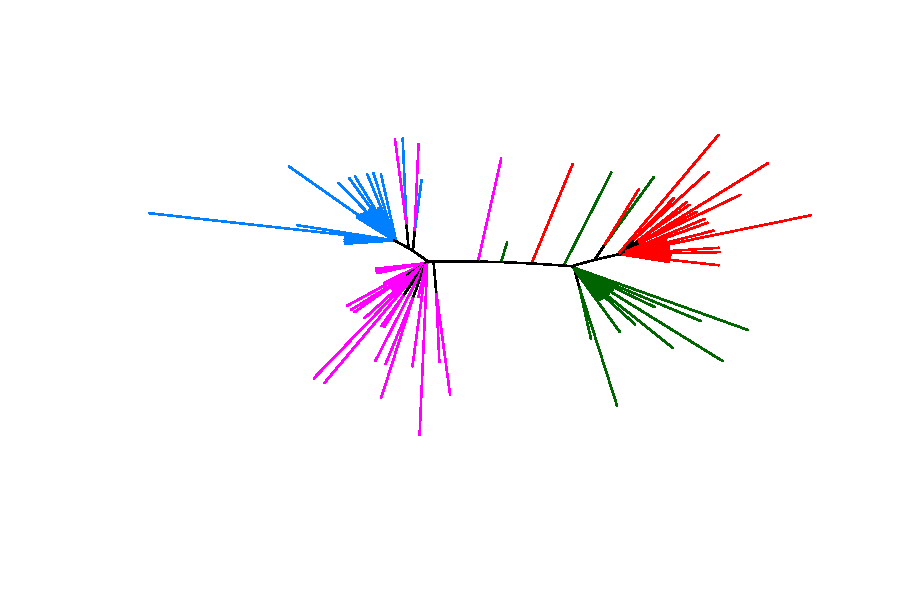
\includegraphics[width=5.0in]{./phyclust-include/f-toynj}
\caption{A NJ tree for the toy dataset.}
\label{fig:toynj}
\end{center}
\end{figure}




\subsection[Using the phyclust() function]{Using the \code{phyclust()} function}
\label{sec:phyclust}
\addcontentsline{toc}{subsection}{\thesubsection. Using the \code{phyclust()}\ function}

We will use the toy dataset to demonstrate the \code{phyclust()} function, which requires two arguments: the data matrix \code{X} and the number of clusters \code{K}.
The optional \code{EMC} argument of \code{phyclust()} is used to pass in model and optimization choices.
By default, the object \code{.EMC} is passed to \code{phyclust()}.
See Section~\ref{sec:emcontrol} for more information about changing the defaults.
In the following example, we use the defaults to fit 4 clusters to the
toy data.
\begin{Code}
> set.seed(1234)
> (ret.1 <- phyclust(X, 4))
Phyclust Results:
code type: NUCLEOTIDE, em method: EM, boundary method: ADJUST.
init procedure: exhaustEM, method: randomMu.
model substitution: JC69, distance: D_JC69.
iter: 37 3158 0, convergence: 0, check.param: 1.
eps: 4.851e-13, error: 0.
N.X.org: 100, N.X.unique: 87, L: 200, K: 4, p: 804, N.seg.site: 127.
logL: -1439, bic: 6581, aic: 4487, icl: 6588
identifier: EE
  Eta: 0.4360 0.01149 0.284 0.2700 
  Tt: 0.003325 
  n.class: 44 1 28 27
> RRand(ret.1$class.id, X.class)
   Rand adjRand  Eindex 
 0.9018  0.7653  0.1655
> class(ret.1)
[1] "phyclust"
\end{Code}

The output of the call to \code{phyclust()} includes
\begin{center}
\begin{tabular}{rl}
	\code{N.X.org}& the number of sequences \\
	\code{N.X.unique}& the number of unique/distinct sequences \\
	\code{L}& for the number of sites \\
	\code{N.seq.site}& for the number of segregating sites \\
	\code{K}& the number of clusters \\
	\code{p}& the number of parameters \\
	\code{logL}& the maximum likelihood value \\
	\code{bic}, \code{aic} and \code{icl}& for BIC, AIC and ICL \\
	\code{identifier}& the model choice for $\vect{Q}_k$ and $t_k$ (see Table~\ref{tab:identifier}) \\
	\code{Eta}& mixing proportions $\vect{\eta}$ \\
	\code{Tt}& $t_k$
\end{tabular}
\end{center}

A quick glance at the results shows that the default settings did not produce good results.
There is a degenerate cluster (only one member), as indicated by the count of members in each of the four classes: \code{n.class}.
The default initialization procedure
is \code{exhaustEM} and the default initialization method is \code{randomMu},
which means it randomly picks 4 sequences to be the cluster centers and
runs the EM algorithm to convergence. While the EM algorithm is guaranteed to converge, it may only find a local optimum.
It is important to try multiple random initializations to improve your chances of finding the global maximum.
The adjusted Rand index \citep{Hubert1985}, \code{adjRand}, which can be used to compare two clusterings, is about 0.7653 when comparing the \code{phyclust()} solution to the true clusters.
It should be $1.000$ for perfect agreement.

The \code{phyclust()} function returns a list object of class
{\color{red} \code{phyclust}}.
You can type \code{str(ret.1)} to get the details of the \code{phyclust}
class, or type \code{?phyclust} to see descriptions of all elements.
Section~\ref{sec:emcontrol} will give more information for controlling
the \code{phyclust()} function.
This object can also be used as input to other functions, for example bootstrapping
and simulations (see Section~\ref{sec:msseqgenphyclust}).




\subsection[Using the .EMControl() function]{Using the \code{.EMControl()} function}
\label{sec:emcontrol}
\addcontentsline{toc}{subsection}{\thesubsection. Using the \code{.EMControl()}\ function}

The \code{.EMControl()} function provides a list object that can be used as argument \code{EMC} to \code{phyclust()}.
With no arguments, it returns the default values. The internal object \code{.EMC}
is a template object holding the defaults. Each element configures some aspect of the evolutionary model,
phyloclust model, initialization, optimization, and EM algorithm. See the help
page for details and visit our website for examples.
\begin{Code}
> ?.EMControl
> ?.EMC
\end{Code}


You can either modify the template \code{.EMC} directly, or use the function
\code{.EMControl()} to generate a new control object.
The following example modifies an object copied from the template.
It changes the initialization method to ``emEM,'' which
yields a better solution than our previous attempt (\code{ret.1}).
The adjusted Rand index is now 1.000, indicating a perfect match between the truth and inferred structures.
\begin{Code}
> EMC.2 <- .EMC
> EMC.2$init.procedure <- .init.procedure[2]
> ### The same as
> ### EMC.2 <- .EMControl(init.procedure = "emEM")
> set.seed(1234)
> (ret.2 <- phyclust(X, 4, EMC = EMC.2))
Phyclust Results:
code type: NUCLEOTIDE, em method: EM, boundary method: ADJUST.
init procedure: emEM, method: randomMu.
model substitution: JC69, distance: D_JC69.
iter: 103 8725 0, convergence: 0, check.param: 1.
eps: 2.753e-14, error: 0.
N.X.org: 100, N.X.unique: 87, L: 200, K: 4, p: 804, N.seg.site: 127.
logL: -1379, bic: 6461, aic: 4367, icl: 6469
identifier: EE
  Eta: 0.2700 0.1898 0.2801 0.2602 
  Tt: 0.003074 
  n.class: 27 19 28 26
> RRand(ret.2$class.id, X.class)
   Rand adjRand  Eindex 
 1.0000  1.0000  0.1209
\end{Code}

Now, we use the function \code{.EMControl()} to generate a
new control that uses ``RndEM'' for initialization.
It also changes the phyloclustering model to use the ``EV'' variant (see Table~\ref{tab:identifier}).
The data was simulated under ``EE'' conditions, so this is an over-parameterized model.
Such models may also tend to infer degenerate clusters,  and again, more initializations may be required for good results.
From the output, we observe
the mixing proprtion \code{Eta} of the second cluster is smaller than others.
In addition, the evolutionary time \code{Tt}  of this cluster is unusually larger compared to the others.
These are both indications of a degenerate cluster, and indeed, no sequences were assigned to this cluster.
\begin{Code}
> EMC.3 <- .EMControl(init.procedure = "RndEM", identifier = "EV")
> ### The same as
> ### EMC.3 <- .EMC
> ### EMC.3$init.procedure <- .init.procedure[3]
> ### EMC.3$identifer <- .identifier[3]
> set.seed(1234)
> (ret.3 <- phyclust(X, 4, EMC = EMC.3))
Phyclust Results:
code type: NUCLEOTIDE, em method: EM, boundary method: ADJUST.
init procedure: RndEM, method: randomMu.
model substitution: JC69, distance: D_JC69.
iter: 104 51836 0, convergence: 0, check.param: 1.
eps: 4.278e-13, error: 0.
N.X.org: 100, N.X.unique: 87, L: 200, K: 4, p: 807, N.seg.site: 127.
logL: -1453, bic: 6621, aic: 4519, icl: 6627
identifier: EV
  Eta: 0.2696 0.01149 0.2844 0.4461 
  Tt: 0.002230 4.75 0.003663 0.003924 
  n.class: 27 0 28 45
> RRand(ret.3$class.id, X.class)
   Rand adjRand  Eindex 
 0.9002  0.7640  0.1698
\end{Code}

There is a convenient function \code{find.best()}
(Section~\ref{sec:msseqgenphyclust}) that is useful for finding
the highest likelihood fit among multiple calls to \code{phyclust()} with
varying arguments.
This function runs \code{phyclust()} repeatedly on
combinations of selected initialization options by updating
an internal \code{EMC} control object in each iteration.
Please be patient, as this function may take some time to complete.




\subsection[The ms+seqgen+phyclust approach]{The ms+seqgen+phyclust approach}
\label{sec:msseqgenphyclust}
\addcontentsline{toc}{subsection}{\thesubsection. The \code{ms+seqgen+phyclust}\ approach \vspace{-0.3cm}}

Model selection includes identifying the number of clusters, type of evolutionary model, and phyloclustering assumptions (Table~\ref{tab:identifier}).
We could use information criteria to choose among models, but the parameter space is mixed continuous and discrete so the theory justifying these critiera does not apply.
A more elaborate procedure to assess the number of clusters
for a dataset is based on the parametric bootstrap
technique and sequential hypothesis testing \citep{Maitra2010}.

The basic idea is to resample datasets from the fitted model using the
functions \code{ms()} and \code{seqgen()},
and refit the resampled dataset by \code{phyclust()}.
The same fitting method is applied to each
dataset, producing a distribution of parameter estimates.
The \code{bootstrap.seq.data()} function is a tool for this procedure;
it takes a fitted model, the output of a previous call to \code{phyclust()}.
The following example bootstraps the toy dataset once assuming $K=2$ clusters.
\begin{Code}
> set.seed(1234)
> ret.4 <- phyclust(X, 2)
> (seq.data.toy.new <- bootstrap.seq.data(ret.4))
code.type: NUCLEOTIDE, n.seq: 100, seq.len: 200.
> (ret.4.new <- phyclust(seq.data.toy.new$org, 2))
Phyclust Results:
code type: NUCLEOTIDE, em method: EM, boundary method: ADJUST.
init procedure: exhaustEM, method: randomMu.
model substitution: JC69, distance: D_JC69.
iter: 30 2947 0, convergence: 0, check.param: 1.
eps: 1.41e-14, error: 0.
N.X.org: 100, N.X.unique: 56, L: 200, K: 2, p: 402, N.seg.site: 69.
logL: -685.3, bic: 3222, aic: 2175, icl: 3222
identifier: EE
  Eta: 0.48 0.52 
  Tt: 0.001354 
  n.class: 48 52
\end{Code}
Output \code{ret.4} is the result from \code{phyclust()},
\code{seq.data.toy.new} is a new dataset bootstrapped from
the model in \code{ret.4}, and \code{ret.4.new} is the fit
of the bootstrapped dataset.
Generally, we need to repeat these steps several times to obtain
a distribution of parameter estimates.
For example, the following code uses $B = 10$ bootstraps to obtain
the distributions of log-likelihood for $K = 1$ and $K = 2$, and
we can perform a likelihood ratio test to assess the number of clusters.
\begin{Code}
> ### This code may take a long time to run.
> set.seed(1234)
> ret.K1 <- find.best(X, 1)
> ret.K2 <- find.best(X, 2)
> (logL.diff <- ret.K2$logL - ret.K1$logL)
[1] 663.2635
> set.seed(1234)
> B <- 10
> boot.logL.diff <- NULL
> for(b in 1:B){
>   seq.data.toy.new <- bootstrap.seq.data(ret.K1)
>   ret.H0 <- find.best(seq.data.toy.new$org, 1)
>   ret.H1.H0 <- find.best(seq.data.toy.new$org, 2)
>   boot.logL.diff <- c(boot.logL.diff, ret.H1.H0$logL - ret.H0$logL)
> }
> boot.logL.diff
 [1] 20.17399 24.94449 25.50644 24.30299 25.94984 19.03801 19.20099 19.40565
 [9] 18.88133 37.16275
> sum(logL.diff < boot.logL.diff)
[1] 0
\end{Code}
Here, the difference of likelihood values \code{logL.idff} is $663.2635$
between models $K = 1$ and $K = 2$.
We bootstrap from a fitted model of $K = 1$,
and it is 0 out of 10 results indicating the $K = 2$ performs
better than $K = 1$. As the $B$ increases, we may more confident to
reject $K = 1$.

